% Only one of the following lines should be used at a time.
%\documentclass[draft,phd,12pt]{psuthesis}
%\documentclass[draft,phd,inlinechaptertoc]{psuthesis}
%\documentclass[draft,ms]{psuthesis}
%\documentclass[draft,honorsdepthead,honors]{psuthesis}
%\documentclass[honors,12pt,draft]{psuthesis}
\documentclass[honors,12pt]{psuthesis}
%\documentclass[draft,secondthesissupervisor,honors]{psuthesis}
%\documentclass[draft,bs]{psuthesis}


%%%%%%%%%%%%%%%%%%%%%%%%%%%%
% Packages we like to use. %
%%%%%%%%%%%%%%%%%%%%%%%%%%%%
\usepackage{amsmath}
\usepackage{amssymb}
\usepackage{amsthm}
\usepackage{exscale}
\usepackage[mathscr]{eucal}
\usepackage{bm}
\usepackage{eqlist} % Makes for a nice list of symbols.
\usepackage[dvipsnames]{color}
\usepackage{psfrag}
\usepackage{varioref}
\usepackage{booktabs}
\usepackage[version=3]{mhchem}
\usepackage[caption=false]{subfig}
\usepackage{url}
\usepackage[final]{graphicx}
%\DeclareGraphicsExtensions{.pdf, .jpg}
\graphicspath{{chapter-1/figures/}{chapter-2/figures/}{chapter-3/figures/}{chapter-4/figures/}{appendix-a/figures/}}
%\usepackage[first,timestamp]{draftcopy}
%\usepackage{rotating}
\usepackage{ctable}
%\usepackage{cite}
\usepackage{lmodern}
\usepackage{textcomp}
\usepackage{setspace}
%\usepackage[citestyle=numeric-comp,backend=bibtex,sorting=none]{biblatex}
%\addbibresource{Biblio-Database.bib}
\doublespacing

%\usepackage{blindtext}

%%%%%%%%%%%%%%%%%%%%%%%%
% Setup caption format %
%%%%%%%%%%%%%%%%%%%%%%%%
%\captionsetup[subfloat]{listofformat=parens}
%\captionsetup{lofdepth=2}

%%%%%%%%%%%%%%%%%%%%%%%%
% Setting for fncychap %
%%%%%%%%%%%%%%%%%%%%%%%%
% Comment out or remove the next two lines and you will get
% the standard LaTeX chapter titles. We like these A LOT
% better.
\usepackage[Lenny]{fncychap}
%\ChTitleVar{\Huge\sffamily\bfseries}
\ChTitleVar{\Huge\rm\bfseries}


%%%%%%%%%%%%%%%%%%%%%%%%%%%%%%%
% Use of the hyperref package %
%%%%%%%%%%%%%%%%%%%%%%%%%%%%%%%
%
% This is optional and is included only for those students
% who want to use it.
%
% To the hyperref package, uncomment the following line:
\usepackage[linktocpage]{hyperref}
\usepackage[all]{hypcap}
%
% Note that you should also uncomment the following line:
\renewcommand{\theHchapter}{\thepart.\thechapter}
%
% to work around some a problem hyperref has with the fact
% the psuthesis class has unnumbered pages after which page
% counters are reset.
\hypersetup{pdftitle={},
	pdfauthor={Klaus Zhang},bookmarksnumbered,pdfstartview=FitH}
%
\labelformat{equation}{\textup{(#1)}}
\labelformat{enumi}{\textup{(#1)}}
%\renewcommand\thesubfigure{(\alph{subfigure})}
%
\let\orgautoref\autoref
\providecommand{\autorefs}
        {\def\equationautorefname{Eqs.}%
         \def\figureautorefname{Figures}%
         \def\subfigureautorefname{Figures}%
         \def\sectionautorefname{Sections}%
         \def\subsectionautorefname{Sections}%
         \def\subsubsectionautorefname{Sections}%
         \def\Itemautorefname{items}%
         \def\tableautorefname{Tables}%
         \orgautoref}
\renewcommand{\autoref}
        {\def\equationautorefname{Eq.}%
         \def\figureautorefname{Figure}%
         \def\subfigureautorefname{Figure}%
         \def\sectionautorefname{Section}%
         \def\subsectionautorefname{Section}%
         \def\subsubsectionautorefname{Section}%
         \def\Itemautorefname{Item}%
         \def\tableautorefname{Table}%
         \orgautoref}				

%%%%%%%%%%%%%%%%%%%%%%%%%%%%%%%%%%%%
% SPECIAL SYMBOLS AND NEW COMMANDS %
%%%%%%%%%%%%%%%%%%%%%%%%%%%%%%%%%%%%
% Place user-defined commands below.



%%%%%%%%%%%%%%%%%%%%%%%%%%%%%%%%%%%%%%%%%
% Renewed Float Parameters              %
% (Makes floats fit better on the page) %
%%%%%%%%%%%%%%%%%%%%%%%%%%%%%%%%%%%%%%%%%
\renewcommand{\floatpagefraction}{0.85}
\renewcommand{\topfraction}      {0.85}
\renewcommand{\bottomfraction}   {0.85}
\renewcommand{\textfraction}     {0.15}

%%%%%%%%%%%%%%%%%%%%%%%%%%%%%%%%%%%%%%%%%%%%%%%%%%%%%%%%%%%%%
% Adjust the equation numbering style to be within sections %
%%%%%%%%%%%%%%%%%%%%%%%%%%%%%%%%%%%%%%%%%%%%%%%%%%%%%%%%%%%%%
\numberwithin{equation}{chapter}

%%%%%%%%%%%%%%%%%%%%%%%%%%%%%%%%%%%%%%%
% Define a narrow environment         %
% (as seen in epslatex documentation) %
%%%%%%%%%%%%%%%%%%%%%%%%%%%%%%%%%%%%%%%
\newenvironment{narrow}[2]{%
\begin{list}{}{%
\setlength{\topsep}{0pt}%
\setlength{\leftmargin}{#1}%
\setlength{\rightmargin}{#2}%
\setlength{\listparindent}{\parindent}%
\setlength{\itemindent}{\parindent}%
\setlength{\parsep}{\parskip}}%
\item[]}{\end{list}}

% ----------------------------------------------------------- %

%%%%%%%%%%%%%%%%
% FRONT-MATTER %
%%%%%%%%%%%%%%%%
% Title
\title{Comparison of Nonlinear Filtering Methods for State Estimation}

% Author and Department
\author{Klaus Zhang}
\dept{Department of Electrical Engineering}
% the degree will be conferred on this date
\degreedate{May 2014}
% year of your copyright
\copyrightyear{2014}

% This command is used for students submitting a thesis to the
% Schreyer Honors College. The argument of this command should
% contain every after the word ``requirements'' that appears on
% the title page. This provides the needed flexibility for
% all the degree types.
\honorsdegreeinfo{Masters of Science \\ in \\ Eletrical Engineering}

% This is the document type. For example, this could also be:
%     Comprehensive Document
%     Thesis Proposal
\documenttype{Thesis}

% This will generally be The Graduate School, though you can
% put anything in here to suit your needs.
\submittedto{The Graduate Falculty}


%%%%%%%%%%%%%%%%%%
% Signatory Page %
%%%%%%%%%%%%%%%%%%
% You can have up to 7 committee members, i.e., one advisor
% and up to 6 readers.
%
% Begin by specifying the number of readers.
\numberofreaders{2}

% For baccalaureate honors degrees, enter the name of your
% honors adviser below.
%\honorsadviser{John D. Mitchell}

% For baccalaureate honors degrees, if you have a second
% Thesis Supervisor, enter his or her name below.
%\secondthesissupervisor{Jeffrey L. Schiano}

% For baccalaureate honors degrees, certain departments
% (e.g., Engineering Science and Mechanics) require the
% signature of the department head. In that case, enter the
% name of your department head below.
%\honorsdepthead{Department Q. Head}

% Input reader information below. The optional argument, which
% comes first, goes on the second line before the name.
%\advisor[Honors Advisor]
        %{Paul Howell}
        %{Professor of Metallurgy}

%\readerone[Honors Advisor]
          %{Elizabeth Walters}
          %{Associate Professor of Art History}

%\readertwo[Faculty Reader]
          %{Digby MacDonald}
          %{Distinguished Professor of Materials Science and Engineering}

%\readerthree[]
            %{Dana Kletchka}
            %{Affiliate Instructor of Art Education}

%\readerfour[Optional Title Here]
%           {Reader Name}
%           {Professor of SomeThing}
%
%\readerfive[Optional Title Here]
%           {Reader Name}
%           {Professor of SomeThing}

% Makes use of LaTeX's include facility. Add as many chapters
% and appendices as you like.
%\includeonly{%
%Chapter-1/Chapter-1,%
%Chapter-2/Chapter-2,%
%Chapter-3/Chapter-3,%
%Chapter-4/Chapter-4,%
%Chapter-5/Chapter-5,%
%Appendix-A/Appendix-A,%
%Appendix-B/Appendix-B%
%}

%%%%%%%%%%%%%%%%%
% THE BEGINNING %
%%%%%%%%%%%%%%%%%
\begin{document}
%%%%%%%%%%%%%%%%%%%%%%%%
% Preliminary Material %
%%%%%%%%%%%%%%%%%%%%%%%%
% This command is needed to properly set up the frontmatter.
\frontmatter

%%%%%%%%%%%%%%%%%%%%%%%%%%%%%%%%%%%%%%%%%%%%%%%%%%%%%%%%%%%%%%
% IMPORTANT
%
% The following commands allow you to include all the
% frontmatter in your thesis. If you don't need one or more of
% these items, you can comment it out. Most of these items are
% actually required by the Grad School -- see the Thesis Guide
% for details regarding what is and what is not required for
% your particular degree.
%%%%%%%%%%%%%%%%%%%%%%%%%%%%%%%%%%%%%%%%%%%%%%%%%%%%%%%%%%%%%%
% !!! DO NOT CHANGE THE SEQUENCE OF THESE ITEMS !!!
%%%%%%%%%%%%%%%%%%%%%%%%%%%%%%%%%%%%%%%%%%%%%%%%%%%%%%%%%%%%%%

% Generates the signature page. This is not bound with your
% thesis.
%\psusigpage

% Generates the title page based on info you have provided
% above.
\psutitlepage

% Generate the signature page
%\psusigpage

% Generates the committee page -- this is bound with your
% thesis. If this is an baccalaureate honors thesis, then
% comment out this line.
%\psucommitteepage

% Generates the abstract. The argument should point to the
% file containing your abstract. 
\setcounter{page}{1}
\thesisabstract{SupplementaryMaterial/Abstract}

% Generates the Table of Contents
\thesistableofcontents

% Generates the List of Figures
%\thesislistoffigures

% Generates the List of Tables
%\thesislistoftables

% Generates the List of Symbols. The argument should point to
% the file containing your List of Symbols. 
%\thesislistofsymbols{SupplementaryMaterial/ListOfSymbols}

% Generates the Acknowledgments. The argument should point to
% the file containing your Acknowledgments. 
%\thesisacknowledgments{SupplementaryMaterial/Acknowledgments}

% Generates the Epigraph/Dedication. The first argument should
% point to the file containing your Epigraph/Dedication and
% the second argument should be the title of this page. 
%\thesisdedication{SupplementaryMaterial/Dedication}{Dedication}



%%%%%%%%%%%%%%%%%%%%%%%%%%%%%%%%%%%%%%%%%%%%%%%%%%%%%%
% This command is needed to get the main part of the %
% document going.                                    %
%%%%%%%%%%%%%%%%%%%%%%%%%%%%%%%%%%%%%%%%%%%%%%%%%%%%%%
\thesismainmatter

%%%%%%%%%%%%%%%%%%%%%%%%%%%%%%%%%%%%%%%%%%%%%%%%%%
% This is an AMS-LaTeX command to allow breaking %
% of displayed equations across pages. Note the  %
% closing the "}" just before the bibliography.  %
%%%%%%%%%%%%%%%%%%%%%%%%%%%%%%%%%%%%%%%%%%%%%%%%%%
\allowdisplaybreaks{
%
%%%%%%%%%%%%%%%%%%%%%%
% THE ACTUAL CONTENT %
%%%%%%%%%%%%%%%%%%%%%%
% Chapters
\documentclass[../zhang_thesis.tex]{subfiles}
\begin{document}

\chapter{Introduction}

Batteries, particularly rechargeable ones, are used extensively in daily life. They provide the energy for such electrical systems as communication, automotive, and renewable power systems. In order to design for and operate these systems, an accurate battery model and a means of simulating the model efficiently is needed. For example, modern battery charge and health management schemes use high-fidelity battery models to track the state of charge (SOC) and state of
health (SOH); this information is then used to predict and optimize the runtime of the battery. However, widely-used chemical batteries have nonlinear capacitive effects, which require the use of a nonlinear filter for accurate prediction of its states in the presence of noise. This thesis explores one possible solutions to this problem by choosing an appropriate battery model and testing the accuracy of various nonlinear filters in determining the SOC through simulation.

%%%%%%%%%%%%%%%%%%%%%%%%%%%%%%%%%%%%%%%%%%%%%%%%%%%%%%%%%%%%%%%

\section{Electrical Characteristics of Rechargeable Batteries}

A high-fidelity battery model has to accurately reproduce the various characteristics of a battery. Most models keep track of the total capacity and SOC in order to predict remaining runtime. More accurate models include nonlinear effects, such as the rate-capacity effect and the recovery effect, along with self-discharge and the effects of ambient temperature. The dynamic electrical attributes, such as the current-voltage (i-v) characteristics and transient responses, can also be
modeled. The remainder of this section defines these characteristics.

The capacity of a battery is the amount of electric charge it can store, measured in the SI unit Ampere-hours (Ah). Commonly, for rechargeable battery specifications, the subunit milliampere-hour (mAh) is used. Related is the available capacity, which is the amount of charge available for use. Due to the electrochemical nature of batteries, a battery's available capacity decreases as the rate of discharge increases, known as the rate-capacity effect. Therefore, the capacity for a
battery is typically stated for a given discharge rate.  Related to this is the recovery effect, so called because when a battery is allowed to rest during an idle period, the battery ``recovers'' available capacity previously lost during discharge due to the rate-capacity effect. Thus, a battery discharged at a high rate until seemingly fully discharged, when allowed to rest, regains a portion of its lost capacity.

Both the rate-capacity effect and the recovery effect can be explained by the electrochemical nature of the battery. During discharge, the concentration of the active material around the electrode is depleted, and the active materials in the depletion region move towards the electrode to reduce the concentration gradient~\cite{chiasserini99}. Because the speed at which the concentration gradient is equalized is limited, the faster the rate of discharge, the less the active material is
replenished, resulting in a decrease in the available capacity. Likewise, when the battery is allowed to rest, the active material gradient has additional time to equalize, and the available capacity is increased.

Closely related to the capacity is the SOC. This thesis defines it as the ratio between the remaining capacity and the maximum capacity, with both capacities measured using the amount of active material within the battery. This definition then denotes the proportion of remaining chemical energy rather the available energy and is unaffected by the rate-capacity and recovery effects. Note that a fully charged battery has an SOC of unity and a fully discharged battery has an SOC of
zero, regardless of the available capacity. Additionally, it is convenient to establish the relationship between the SOC of the battery and its open-circuit voltage $V_{OC}$, which is useful for simulation of the i-v characteristics and transient responses. $V_\text{OC}$ can be thought as the limit of the measured battery voltage after recovery.

Other more minor effects that are usually incorporated into models are self-discharge, the effect of ambient temperature, and aging. Self-discharge refers to an idle battery decreasing its SOC over time due to internal chemical reactions. It is dependent on the type of battery, SOC, ambient temperatures, and other factors. The ambient temperature has effects on the internal resistance of the battery and the self-discharge rate. Commonly, the battery is designed to operate with a narrow range of temperatures. Below the operating temperature range, the internal resistance increases, decreasing the capacity. Above the operating range, the internal resistance decreases, not only increasing the capacity but also the self-discharge rate; thus, the actual capacity is lowered due to the increased self-discharge. Aging refers to the decrease in battery performance measures, such as capacity, self-discharge, and internal resistance, over time due to unwanted chemical reactions. In practice, aging is indicated by the SOH, defined as the ratio between the current maximum capacity and that of a new battery. The SOH threshold at which the battery performance is considered too degraded varies by application.

%This thesis studied the prediction of the SOC of a battery using noisy measurements of its current and voltage. To do so accurately for a general load, incorporation of the rate-capacity and recovery effects as well as the transient i-v characteristics is desirable. Furthermore, it is useful to have a model easily tunable for different battery types. The following section reviews the characteristics of different battery models and chooses the one most suitable for the purposes of this study.

%%%%%%%%%%%%%%%%%%%%%%%%%%%%%%%%%%%%%%%%%%%%%%%%%%%%%%%%%%%%%%%

\section{Battery Models}

This thesis studied the predition of the SOC of a battery given knowledge of the resistive load on the battery as well as noisy measurements of the voltage across its terminals. In order to do so for a general load profile, incorporation of the rate-capacity and recovery effects as well as the transient i-v characteristics is desirable. Furthermore it is useful to have a model easily tunable for different battery types. This section reviews the characteristics of major types of
battery models. Battery models can be divided into five categories, namely electrochemical, computational intelligence, analytical, stochastic, and electrical-circuit. The remainder of this section reviews each type and determines the most suitable battery model for this study.

\subsection{Electrochemical}

Electrochemical models are describe the chemical processes that place in the battery in great detail. These are generally the most accurate, but they require in-depth knowledge of the chemical processes to create and impose large computational costs~\cite{jongerden09}. One of the most widely known electrochemical models was developed by Doyle, Fuller, and Newman for lithium and lithium-ion batteries using noninvasive voltage-current cycling
experiments~\cite{doyle93,fuller94,fuller94b}. It consists of six coupled, nonlinear differential equatons that capture lithium diffusion dynamics and charge transfer kinetics. The model is able to predict i-v response and provides a design guide for thermodynamics, kinetics, and transport across electrodes. A implementation of their model in Fortran, called Dualfoil, is available for free online.\footfullcite{newman98} The program needs more than 60 parameters along with the load profile
in order to compute the battery properties. Setting the parameters requires detailed knowledge of the battery, but the result of the program is highly accurate. Other battery models are often compared to it rather than to experimental results.

\subsection{Computational Intelligence}

Computational intelligence is a brance of computer science interested in problems that require the intelligence of humans and animals to solve. One of the earliest definitions by Bezdek states that computational intelligent systems use pattern recognition on low-level, numerical data and do not use knowledge as with artificial intelligence~\cite{bezdek92,bezdek94}. Methods such as neural networks, fuzzy systems, and evolutionary computation are commonly classified as computational
intelligence. Battery models using such methods as neural networks~\cite{ogorman98,capizzi11}, support vector machines~\cite{wang06}, and hybrid neural-fuzzy models~\cite{shen02} have been studied. These models learn the nonlinear relationships between battery properties, such as SOC, current, voltage, and temperature, through a computationally costly training process. However, once trained, they incur a much lower cost and can achieve comparable accuracy to electrochemical
models.

\subsection{Analytical}

Analytical models are simplified electrochemical models that trade off accuracy for simplicity. One of the simplest such models is Peukert's law for lead-acid batteries, which states that for a one-ampere discharge rate~\cite{doerffel06}
\begin{equation}
C_p = I^k t,
\end{equation}
where $C_p$ is the capacity at a one-ampere discharge rate in Ah, $I$ is the discharge current in A, $t$ is the time to discharge the battery in hours, and $k\ge 1$ is the dimensionless Peukert constant, typically between 1.1 and 1.3 for a lead-acid battery. The constant $k$ only equals unity for an ideal accumulator, so for real batteries, $k$ is always greater than unity. Thus, for a given increase in the discharge current, the discharge time decreases by a proportionally greater
amount. Therefore, the effective, or available, capacity $C\times t$ is reduced. Peukert's law can be extended to some other battery chemistries, such as lithium-ion. Note that Peukert's law only models the rate-capacity effect and not the recovery effect. More complicated models, such as the kinetic battery model and the diffusion model, are able to describe both effects.

The kinetic battery model (KiBaM), initially created for large lead-acid batteries, describes the battery as a kinetic process, using two charge wells for the bound and available charges connected by a valve whose flow rate is proportional to the height difference between the wells~\cite{manwell93}. The change of charge in the wells is given by
\begin{equation}
    \begin{cases}
        \dfrac{dy_1}{dt} = -I + k \left( h_2 - h_1 \right) \\
        \dfrac{dy_2}{dt} = -k \left( h_2 - h_1 \right),
    \end{cases}
    \label{eq:kibam}
\end{equation}
where $y_1,y_2$ are the charges, $h_1,h_2$ are the heights of the wells, the parameter $k$ controls the rate of charge flow between the wells, and $I$ is the applied load. The flow rate of the valve should be lower than the typical discharge rate of the battery. During discharge from the available-charge well, the bound charges flow through the valve to equalize the heights of the two wells. It can be seen that for slower discharge rates, more charge flows through the valve and the effective
capacity increases. Likewise, during idle periods for the battery, the available charge increases.

Related to the KiBaM is the diffusion model, which describes the movement of the ions in the electrolyte of a lithium-ion battery~\cite{rakhmatov01}. Like in the kinetic battery model, the difference in the concentration of adjacent ions along the length of the battery determines the diffusion rate of the ions. The available charges are those ions directly touching the electrode of the battery. It can be seen that the KiBaM is a first-order approximation of the diffusion
model~\cite{jongerden09}, since the individual ions in the diffusion model are replaced by two charge wells in the KiBaM.

\subsection{Stochastic}

Stochastic models describe the discharging and the recovery effect as stochastic processes. The first models were developed by Chiasserini and Rao and based on discrete-time Markov chains~\cite{chiasserini99b}. They studied two models of a battery in a communication device that transmitted packets. The simpler model described the battery as a discrete-time Markov chain with $N+1$ states, numbered from $0$ to $N$ and corresponding to the number of charge units available in the battery.
Transmitting one packet requires one charge unit of energy. Thus, in continuous transmission, $N$ packets can be sent. At every time step, a charge unit is either consumed with probability $a_1=q$ or recovered with probability $a_0=1-q$. The battery is considered empty when the $0$ state is reached or when a theoretical maximum of $T$ charge units have been consumed. The second model is an extension of the first, allowing for more than one charge unit to be consumed in a time step, modeling
more bursty usage. Additionally, the battery has a non-zero probability of staying in the same charge state, indicating no consumption or recovery during a time step. Chiasserini and Rao extended their model further in following papers by adding state and phase dependence~\cite{chiasserini99,chiasserini01,chiasserini01b}. The state number is the number of charge units, and the phase number is the number of consumed charge units. Having fewer charge units decreases the probability of
recovery, while having more consumed charge units increases the probability of recover. Using these models, one can model different loads by setting the transitions probabilities. However, the order of the transitions is uncontrollable, so it is impossible to model fixed load patterns and compute their impact on battery life.

Chiasserini and Rao mainly investigated the gain $G$ in transmitted packets using a pulsed discharge relative to using a constant discharge, defined as $G=m/N$, where $m$ is the mean number of transmitted packets. The gain increases when the load decreases, due to an increase in the recovery probability. Additionally, the gain increases for lower discharge demand rates and higher current densities. These load profiles result in discharge currents close to the specified limits of the battery, causing the
available capacity to decrease overly quickly. Therefore, the recovery effect is especially strong for these cases during pulsed discharge, greatly increasing the gain. Chiasserini and Rao compared the computation of the gain parameter for different current densities and demand rates using the stochastic model to that of the electrochemical model of Doyle et al. They found an average deviation of 1\% and a maximum deviation of 4\%. This shows that the stochastic model accurately describes battery behavior during pulsed discharge. However, this model is only able to compute relative lifetimes.

In 2005, Rao et al.~\cite{rao05} proposed a stochastic battery model based on the Kinetic Battery Model (KiBaM) of Manwell and McGowan. This stochastic KiBaM was for a nickel-metal hydride (NiMH) battery. The differential equations governing the original KiBaM were modified to include an extra factor $h_2$ governing the flow of charge between the wells. This changes \autoref{eq:kibam} into
\begin{equation}
    \begin{cases}
        \dfrac{dy_1}{dt} = -I + k_s h_2 \left( h_2 - h_1 \right) \\
        \dfrac{dy_2}{dt} = -k_s h_2 \left( h_2 - h_1 \right),
    \end{cases}
\end{equation}
This change causes the recovery effect to weaken as the remaining charge decreases. The stochastic model was also modified to allow the possibility of no recovery during idle periods. The stochastic KiBaM describes the battery using a discrete-time, transient Markov process. The states are labeled with the parameters $(i,j,t)$, with $i$ and $j$ representing the discrete charge levels of the available and bound charge wells and $t$ representing the length of the current idle period.
Like the stochastic model of Chiasserini and Rao, it is impossible to fully model a real-life discharge pattern using the stochastic KiBaM. Rao et al.\ compared the results of their model with experimental results using an AAA NiMH battery. Two sets of experiments were conducted, the first with varying frequency of the load and a 50\% duty cycle and the second with varying off-time and a constant on-time. Their model accurately predicted the lifetime and delivered charge from the
battery, with a maximum error of 2.65\%.

\subsection{Electrical-Circuit}

Electrical-circuit models for batteries developed from the discovery of capacitative effects at the electrode-electrolyte interface. Helmholtz first proposed the existence of a double layer of charge at the interface in 1879. In 1899, Warburg proposed a series resistance and capacitance circuit model with an infinitely low current density. The Warburg capacitance $C_W$ named after him varies inversely with the square root of the frequency~\cite{geddes97}. In 1947, Randles proposed a model
consisting of a double-layer polarization capacitance $C_p$ in parallel with the series combination of a resistor $R$ and a capacitance $C$~\cite{randles47}. In 1994, Kovacs improved Randles circuit with the addition of Warburg impedence $Z_W$ replacing the capacitance $C$ and the solution resistance $R_s$ in series with the original Randles circuit~\cite{kovacs95}. In addition, he renamed $C_p$ to the double layer capacitance $C_{dl}$ and $R$ to the charge-transfer resistance
$R_{ct}$. These proposals came from a desire to represnt impedance spectra created using electrochemical impedance spectroscopy (EIS). The various elements in the models represent the different processes within a battery, which have different time constants. While these attempts model the impedance and, thus, account for the nonlinear rate-capacity and recovery effects, they do not consider the capacity and self-discharge of the battery.

%\begin{figure}[htb]
%    \centering
%    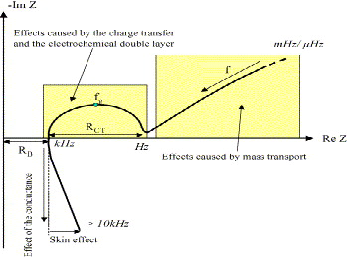
\includegraphics[width=0.8\textwidth]{nyquist_plot_batt}
%    \caption{Illustrative Nyquist plot of a battery~\cite{jossen06}. \emph{[Quite low quality from screen capture of article preview. I can recapture for better quality or recreate it.]}}
%    \label{fig:nyquist_plot_batt}
%\end{figure}

%\begin{figure}[htb]
%    \centering
%    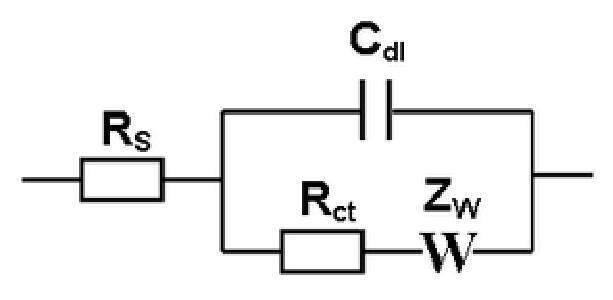
\includegraphics[width=0.6\textwidth]{randles_circuit}
%    \caption{Randles' equivalent circuit.}
%    \label{fig:randles_circuit}
%\end{figure}

In 1993, Hageman created simplified electrical-circuit models using PSpice for nickel-cadmium (NiCd), lead-acid, and alkaline batteries~\cite{hageman93}. The circuits shared the common elements of
\begin{enumerate*}[label=\emph{\roman*})]
\item a capacitor that represents the battery capacity,
\item a discharge rate normalizer that determines the additional capacity loss at high discharge rates,
\item a circuit that discharges the battery,
\item a lookup table of battery voltage versus SOC, and
\item a resistor that represents the battery's internal resistance~\cite{hageman93,hageman97}.
\end{enumerate*}
In addition, battery models for NiCd batteries simulated the thermal effects under high discharge rates. The main lookup table is formed by discharging a battery at a low rate at a constant current (20 to 200 hours). At high discharge rates, the discharge rate normalizer reduces the battery voltage below the value from looking up the SOC in the table. This normalizer is implemented using additional lookup tables. These circuit models are much simpler than electrochemical models, but they
are also less accurate with an approximate error of 10\%. Furthermore, creation of the lookup tables requires considerable data. These circuit-based models are mainly concerned with modeling the remaining discharge time and are referred to as runtime-based models.

In 2006, Chen and Rinc\'on-Mora proposed a combination of a runtime-based model and a impedance-based model consisting of a series resistor and two parallel resistor-capacitor networks~\cite{chen06}. The elements of the impedance part of the model had parameters that depended on the SOC. Additionally, the runtime model included a resistance that modeled the self-discharge rate. Their proposed model has the advantage of accurate prediction of the SOC using the runtime-based portion while also modeling
nonlinear transient effects, such as the rate-capacity and recover effects, with the impedance-based portion. Furthermore, the battery data can be collected using EIS measurements, which requires neither detailed knowledge of the battery chemistry nor lengthy, low-rate discharge experiments.

\subsection{Evaluation}

Of the model types, only some are fit for use with filtering algorithms. The computational-intelligence and stochastic models do not model the dyanmics of the battery system, so they cannot be used. The electrochemical models, the related analytical models, and the electrical-circuit models describe the system dynamics and the nonlinear rate-capacity and recovery effects. However, only the electrical-circuit model has the advantage of modeling the internal impedance of the battery,
which is useful in the design of battery systems. Of the electrical-circuit models, the proposal by Chen and Rinc\'on-Mora is best suited for the purposes of this thesis since it is the only one discussed by this paper that describes both the capacity and the transient effects. Therefore, their proposal is used for the simulation of the battery and comparing the performance of different filters.

%%%%%%%%%%%%%%%%%%%%%%%%%%%%%%%%%%%%%%%%%%%%%%%%%%%%%%%%%%%%%%%

\section{Nonlinear Filtering Methods}

Filtering refers to the methodology for estimating the state of a time-varying system that is indirectly observed through noisy measurements. Specifically, the current state is estimated from the current and previous measurements. The state of a system is a group of dynamic variables that evolve through time, and its evolution through time is governed by a dynamic system, perturbed by process noise. The measurements are functions of the state and measurement noise. A battery can be modeled as a
time-varying system, with state variables that describe such states as the SOC and the SOH. The measurements are typically the voltage and the current. Note that this thesis uses a resistive load instead of the current, because this is more realistic from a usage standpoint. Additionally, the SOH is not considered by this thesis. The dynamic system for the battery is described in more detail in the following chapter.

For linear systems, the optimal filtering solution with respect to the minimum mean squared error (MMSE) is given by the least squares solution, meaning the optimal least squares solution equals the posterior mean. A closed form solution to the discrete-time linearing filtering problem is given by the Kalman filter~\cite{kalman60}, which is a linear MMSSE (LMMSE) filter. Under the assumption that the noises are Gaussian, the posterior distribution is also Gaussian and numerical
approximations are unnecessary. The Kalman filter has a prediction phase and an update phase. The prediction phase estimates the current state using the state estimate from the previous time step. The update phase refines the state estimate using the current measurement.

For nonlinear systems, optimal filtering solutions are generally intractable, so various numerical approximation methods have been developed, mainly classified in three groups: function approximation, moment approximation, and stochastic model approximation~\cite{li04}. Function approximation techniques approximate the nonlinear dynamic and measurement processes, commonly using the Taylor series expansion. A moment approximation technique uses a representative
set of sample points and calculates integrals as weighted averages. Stochastic model approximation simplifies the original nonlinear stochastic system to a linear system so that linear filtering results are applicable.

Note that the choice of discretization method tends to depend on the filter, especially for highly nonlinear systems. Therefore, the simulations used a continuous-discrete (mixed) time system, with the form
\begin{align}
    \mathbf{\dot{x}}(t) &= \vf(\mathbf{x}(t),\mathbf{u}(t),\mathbf{w}(t)) \label{eq:gen_ct_f} \\
    \mathbf{z}_k &= \vh(\mathbf{x}(t_k),\mathbf{u}(t_k),\mathbf{v}(t_k)),
\end{align}
where $\vx$, $\vu$, $\mathbf{z}$, $\mathbf{w}$, and $\mathbf{v}$ are the vectors of the states, the inputs, the measurements, the process noises, and the measurement noises, respectively. For simplicity of simulation, the input $\mathbf{u}(t)$ is assumed to be constant over each time step so that $\mathbf{u}(t)=\mathbf{u}(t_k)$ for $t_k\le t < t_{k+1}$. For the prediction phase, the continuous-time dynamics were solved numerically, with each filter using different approximation
techniques. The state error covariances are also approximated numerically. Then, the updates were performed based on the update of the linear Kalman filter.

Furthermore, note that the system is extremely stiff for some inputs $\mathbf{u}$, which can be seen from the stiffness ratio based on the ratio of the largest eigenvalue of $F$ to its smallest eigenvalue, where $F$ is the jacobian of the dynamics $\vf(\mathbf{x},\mathbf{u})$; when the stiffness ratio is much greater than unity, the system is stiff~\cite{lambert91,brugnano11}. From EIS studies of batteries, the major chemical processes have widely differing time constants; low frequency
mass transport effects like diffusion are on the order of $10^{-6}$ to $10^0$ Hz, middle frequency effects caused by charge transfer and the electrochemical double layer are on the order of $10^0$ to $10^3$ Hz, and the high frequency conductance and skin effects are on the order of $10^3$ to $10^4$ Hz~\cite{jossen06}. Therefore, the approximate stiffness ratio is $10^{10} \gg 1$, and the system is stiff. As a result of the stiffness, any numerical integration method needs to be A-stable,
i.e.\ the method converges for all systems whose eigenvalues have negative real parts. For example, simulation results show that the fourth-order Runge-Kutta method diverges even at step sizes $<10^{-2}$ seconds.

S\"arkk\"a and Solin state that a linearized discretion approach, in which the continuous-time system is first discretized and then approximated as Gaussian, tends to work better than a discretized linearization approach, in which the system is first approximated as a Gaussian process and then discretized~\cite{sarkka12}. This thesis follows this guideline and performs the prediction using linearized approximations of a discretization of the continuous-time dynamics. The specifics of the
linearized discretion approach for each filter along with their general implementation are discussed in the remainder of this chapter.

\subsection{Function Approximation}

%The Taylor series expansion for a function $f(\mathbf{x},t)$ at $\hat{\mathbf{x}}$ is given by
%\begin{equation}
%    f(\mathbf{x},t) \approx f(\hat{\mathbf{x}},t) + f'(\hat{\mathbf{x}},t) (\mathbf{x}-\hat{\mathbf{x}}) + \frac{1}{2!} f''(\hat{\mathbf{x}},t) (\mathbf{x}-\hat{\mathbf{x}})^2 + \cdots + \frac{1}{n!} f^{(n)}(\hat{\mathbf{x}},t) (\mathbf{x}-\hat{\mathbf{x}})^n,
%\end{equation}
%where
%\begin{equation}
%    f^{(n)}(\hat{\mathbf{x}},t) = \left. \frac{\partial^n f}{\partial \mathbf{x}^n} \right|_{\mathbf{x}=\hat{\mathbf{x}}}.
%\end{equation}
%Typically, the distance between $\mathbf{x}$ and $\hat{\mathbf{x}}$ is denoted by $\tilde{\mathbf{x}} = \mathbf{x} - \hat{\mathbf{x}}$.

One of the most popular nonlinear filters is the extended Kalman filter (EKF), which approximates the nonlinear state and measurement equations, typically using Taylor series expansion. The standard Kalman filter formulas are used for the update. For the discrete-time EKF, Taylor series expansion can be directly used on the system dynamics to linearize them. For the mixed-time system of this study, a linearized discretization approach proposed by Mazzoni~\cite{mazzoni07} is used, in
which the dynamics are first discretized and then approximated using Taylor series expansion. This approach has the advantage of A-stability. The discretization is performed using the trapezoidal approximation (Heun's method) of \autoref{eq:gen_ct_f}. For convenience, denote the value of a quantity at time $t_k$ using the subscript $k$ and assume that $\delta=t_{k+1}-t_k$ is the time step. Additionally, a subscript of $k|k-1$ indicates the value at time $t_k$ given the information at
$t_{k-1}$. Then, the approximation produces
\begin{equation}
    \vx_{k+1} \approx \vx_k + \frac{1}{2} \big( \vf(\vx_k) + \vf(\vx_{k+1}) \big) \delta.
\end{equation}
The vector field $\vf$ at $\vx_{k+1}$ is approximated by first-order Taylor expansion around $\vx_k$, giving
\begin{equation}
    \vx_{k+1} \approx \vx_k + \vf(\vx_k)\delta + \frac{1}{2} F(\vx_k) \left( \vx_{k+1} - \vx_k \right) \delta,
\end{equation}
where $F(\vx_k)$ is the Jacobian of $\vf$ at $\vx_k$. Solving for $\vx_{k+1}$ yields
\begin{equation}
    \vx_{k+1} \approx \vx_k + \left( I - F(\vx_k) \frac{\delta}{2} \right)^{-1} \vf(\vx_k) \delta,
\end{equation}
with the identity matrix $I$. This Taylor-Heun scheme uses linear Taylor expansion of $f$ rather than then Euler prediction of the standard Heun scheme. This numerical integration scheme is convergent with order $\mathcal{O}(\delta^2)$ and A-stable~\cite{mazzoni07}. For the state error covariance ODE given by
\begin{equation}
    \dot{P} = F(\vx) P + P F^\top(\vx) + L(\vx) Q(\vx) L^\top(\vx),
\end{equation}
where $Q$ is the covariance of the error variables and $L$ is the Jacobian of $\vf$ with respect to the state error variables $\mathbf{w}$, the numerical integration method should have the key features of being consistent with the same order as the Taylor-Heun scheme, able to process nonautonomous differential equations, and A-stable. Mazzoni proposed using a modified Gauss-Legendre formula with an implicit increment rule, producing
\begin{gather}
    P_{k+1} \approx P_k + M_\tau \left( F(\vx_\tau) P_k + P_k F^\top(\vx_\tau) + L(\vx_\tau) Q(\vx_\tau) L^\top(\vx_\tau) \right) M_\tau^\top \delta, \\
    \intertext{with}
    M_\tau = \left( I - F(\vx_\tau) \frac{\delta}{2} \right)^{-1} \quad \text{and} \quad \tau = t_k + \frac{\delta}{2}.
\end{gather}
The value of $\vx_\tau$ can be interpolated from $\vx_k$ and $\vx_{k+1}$ with a precision of $\mathcal{O}(\delta^3)$ using series expansion, producing
\begin{equation}
    \vx_\tau \approx \frac{1}{2} \left( \vx_k + \vx_{k+1} - F(\vx_k) f(\vx_k) \frac{\delta^2}{4} \right).
\end{equation}
This modified Gauss-Legendre approximation is A-stable, consistent with order $\mathcal{O}(\delta^2)$, and ensures the positive definiteness of the resultant error covariance matrix~\cite{mazzoni07}. This numerical integration can be repeated multiple times with a smaller step size should greater accuracy be desired. The update equations for the EKF come from the LMMSE filter and are
\begin{align}
    K_k &= P_{k|k-1} H_k^\top \left( H_k P_{k|k-1} H_k^\top + M(\vx_k) R(\vx_k) M^\top(\vx_k) \right)^{-1} \\
    \vx_{k|k} &= \vx_{k|k-1} + K_k \big( \mathbf{z}_k - \vh(\vx_{k|k-1}) \big) \\
    P_{k|k} &= (I - K_k H_k) P_{k|k-1},
\end{align}
where $R$ is the covariance of the measurement error variables, $M$ is the Jacobian of $\vf$ with respect to the measurement error variables $\mathbf{v}$, and $H_k$ is the Jacobian of $\vf$ at $\vx_{k|k-1}$.

\subsection{Moment Approximation}

In moment approximation, the mean, covariance, and possibly higher-order moments are approximated directly, rather than approximating the nonlinear integrations of expectations. Of the numerical moment approximation methods, two of the best known are the unscented Kalman filter (UKF) and the cubature Kalman filter (CKF). Note that the CKF is a special case of the UKF, but they are considered separately by this study.

In order to handle the mixed-time system, the It\^o-Taylor expansion with a strong order of 1.5 (IT-1.5) proposed by Arasaratnam et al.\ is used to discretize the stochastic differential equations (SDE) for numerical integration~\cite{arasaratnam10}. In the context of Gaussian filtering, the weak order of convergence is more important, because the moments of the distributions and not the functionals of the path are of importance. Thus, the IT-1.5 expansion is equivalent to the weak It\^o-Taylor expansion
of order 2.0~\cite{kloeden99}, which was proposed as a SDE discretization method for target tracking applications by Morelande and Gordon~\cite{morelande05}. For a SDE of the form
\begin{equation}
    d\vx(t) = \vf(\vx(t),t)dt + \sqrt{Q} d\mathbf{\beta}(t),
\end{equation}
Arasaratnam et al. gives the IT-1.5 expansion as~\cite{arasaratnam10}
\begin{equation}
    \vx_{k+1} = \vx_k + \delta \vf(\vx_k) + \frac{\delta^2}{2} \big( \mathbb{L}_0 \vf(\vx_k) \big) + \sqrt{Q} \mathbf{w} + \big( \mathbb{L} \vf(\vx_k) \big) \mathbf{y},
\end{equation}
where
\begin{align}
    \mathbb{L}_0 & = \frac{\partial}{\partial t} + \sum_{i=1}^n \vf_i \frac{\partial}{\partial \vx_i} + \frac{1}{2} \sum_{j,p,q=1}^n \sqrt{Q}_{p,j} \sqrt{Q}_{q,j} \frac{\partial^2}{\partial \vx_p \partial \vx_q} \\
    \mathbb{L}_j & = \sum_{i=1}^n \sqrt{Q}_{i,j} \frac{\partial}{\partial \vx_i}
\end{align}
and $(\mathbf{w},\mathbf{y})$ are a pair of correlated Gaussian random variables generated from a pair of independent standard Gaussian random variables. In the absense of noise, the discretization is
\begin{equation}
    \vx_{k+1} = \vf_d(\vx_k) = \vx_k + \delta \vf(\vx_k) + \frac{\delta^2}{2} \big( \mathbb{L}_0 \vf(\vx_k) \big).
\end{equation}
It can be shown that the expected value of the state is given by
\begin{equation}
    \vx_{k+1} = \int_{\mathcal{R}^n} \vf_d(\vx_k) \mathcal{N}(\vx_k;\hat{\vx}_{k|k},P_{k|k})\,\mathrm{d}\vx_k.
\end{equation}
The propagation of the covariance matrix is given by
\begin{align}
    P_{k|k} = \begin{multlined}[t] \int_{\mathcal{R}^n} \vf_d(\vx_k) \vf_d^\top(\vx_k) \mathcal{N}(\vx_k;\hat{\vx}_{k|k},P_{k|k})\,\mathrm{d}\vx_k + \frac{\delta^3}{3} \big( \mathbb{L}\vf(\vx_k) \big) \big( \mathbb{L}\vf(\vx_k) \big)^\top \\ 
    + \frac{\delta^2}{2} \left[ \sqrt{Q} \big(\mathbb{L}\vf(\vx_k)\big)^\top + \big(\mathbb{L}\vf(\vx_k)\big)^\top \sqrt{Q} \right] - (\hat{\vx}_{k|k})(\hat{\vx}_{k|k})^\top + \delta Q.
    \end{multlined}
\end{align}
The Gaussian integrals can then be approximated using the unscented transform in the UKF and the third-degree cubature rule in the CKF. It can be seen that the IT-1.5 expansion needs to evaluate the first and second order derivatives of the dynamic system, which makes these moment approximation methods no longer derivative-free. There is also a performance hit associated with the evaluations of the derivatives. However, the advantages are greater stability of the filter and impproved numerical accuracy, which are necessary for the stiff system.

The following two sections discuss the implementation of the UKF and CKF in mixed-time using IT-1.5 for the propagation of the dynamics.

\subsubsection{Unscented Kalman Filter}

The UKF is an efficient, generally derivative-free filtering algorithm that relies on the unscented transformation (UT). The UT is useful for forming the Gaussian approximation to the joint distribution of random variables $x$ and $y$ for $x\sim \mathcal{N}(m,P)$ and $y=g(x)$, where $x\in\mathbb{R}^n$, $y\in\mathbb{R}^m$, and $g:\mathbb{R}^n\mapsto\mathbb{R}^m$ is a nonlinear function. Then, the first and second moments corresponding to the mean and covariance can be
easily found. Specifically, suppose the Gaussian approximation of the joint probability density of $x$ and $y$ has the form
\begin{equation}
    \begin{bmatrix} x \\ y \end{bmatrix} = \mathcal{N} \left( \begin{bmatrix} m \\ \mu_U \end{bmatrix}, \begin{bmatrix} P & C_U \\ C_U^\top & S_U \end{bmatrix} \right).
\end{equation}
Then, the UT picks $2n+1$ sample points $\{x_i\}$, commonly known as sigma points, along with the same number of weights $\{w_i\}$, as follows~\cite{sarkka07}. First, the sigma points are chosen from the columns of the matrix $\sqrt{(n+\lambda)P}$, giving
\begin{align}
    x^{(0)} & = m_x \\
    x^{(i)} & = m_x + \left[ \sqrt{(n+\lambda)P} \right]_i, \quad i=1,\dots,n \\
    x^{(i)} & = m_x - \left[ \sqrt{(n+\lambda)P} \right]_{i-n}, \quad i=n+1,\dots,2n
\end{align}
with the weights
\begin{align}
    W_0^{(m)} & = \frac{\lambda}{n+\lambda} \\
    W_0^{(c)} & = \frac{\lambda}{n+\lambda} + (1-\alpha^2+beta) \\
    W_i^{(m)} & = W_i^{(c)} = \frac{1}{2(n+\lambda)}, \quad i=1,\dots,2n.
\end{align}
The parameter $\lambda$ is defined as
\begin{equation}
    \lambda = \alpha^2 (n+\kappa) - n,
\end{equation}
and the constants $\alpha$, $\beta$, and $\kappa$ are parameters of the method. For the UKF, $\alpha$ is a small positive number, e.g.\ $10^{-3}$, $\beta=2$ is ideal for a Gaussian distribution, and $\kappa$ is typically 0. Each sigma point is transformed by
\begin{equation}
    y^{(i)} = g(x^{(i)}, \quad i=0,\dots,2n.
\end{equation}
Then, moments are approximated by
\begin{align}
    \mu_U & = \sum_{i=0}^{2n} W_i^{(m)} y^{(i)} \\
    S_U & = \sum_{i=0}^{2n} W_i^{(c)} ( y^{(i)} - \mu_U ) ( y^{(i)} - \mu_U )^\top \\
    C_U & = \sum_{i=0}^{2n} W_i^{(c)} ( x^{(i)} - m ) ( y^{(i)} - \mu_U )^\top.
\end{align}
The square root of the positive definite matrix P is defined as a matrix $A$ such that $P=AA^\top$. Note that $A$ is not unique. For performance reasons, the Cholesky factorization is typically used. The UT algorithm is denoted as
\begin{equation}
    [\mu_U,S_U,C_U] = \mathrm{UT}(g,m,P).
\end{equation}
Then, for the discretized system
\begin{align}
    \vx_k & = \vf_d(\vx_{k-1}) + \mathbf{q}_{k-1} \\
    \mathbf{y}_k & = \mathbf{h}(\vx_k) + \mathbf{r}_k,
\end{align}
where $\mathbf{q}_k\sim\mathcal{N}(0,Q_{k})$ and $\mathbf{r}_k\sim\mathcal{N}(0,R_{k})$, the prediction and update steps for the UKF can be written as
\begin{align}
    [m_k^{-},\tilde{P}_k] & = \mathrm{UT}(\vf_d,m_{k-1},P_{k-1}) \\
    P^{-}_k & = \tilde{P}_k + Q_{k-1} \\
    [\mu_k,\tilde{S}_k,C_k] & = \mathrm{UT}(\mathbf{h},m_k^{-},P^{-}_k) \\
    S_k & = \tilde{S}_k + R_k \\
    K_k & = C_k S_k^{-1} \\
    m_k & = m_k^{-} + K_k (y_k-\mu_k) \\
    P_k & = P^{-}_k - K_k S_k K_k^\top.
\end{align}
The discretized dynamics are those from the previous section.

\subsubsection{Cubature Kalman Filter}

The CKF uses the cubature rule rather than the UT to approximate the Gaussian integrals. For the CKF, $2n$ sigma points are chosen, giving~\cite{arasaratnam10}
\begin{align}
    x^{(i)} & = m_x + \left[ \sqrt{nP} \right]_i, \quad i=1,\dots,n \\
    x^{(i)} & = m_x - \left[ \sqrt{nP} \right]_{i-n}, \quad i=n+1,\dots,2n.
\end{align}
The weights are uniformly $W_i=1/2n$. Thus, the moments are approximated by
\begin{align}
    \mu_U & = \frac{1}{2n} \sum_{i=0}^{2n} y^{(i)} \\
    S_U & = \frac{1}{2n} \sum_{i=0}^{2n} ( y^{(i)} - \mu_U ) ( y^{(i)} - \mu_U )^\top \\
    C_U & = \frac{1}{2n} \sum_{i=0}^{2n} ( x^{(i)} - m ) ( y^{(i)} - \mu_U )^\top.
\end{align}
It can be seen that the cubature rule is a special case of the UT with $\alpha=1$, $\beta=0$, and $\kappa=0$. This choice of parameters results in $W_0=0$, eliminating one of the sigma points. The prediction and update steps then proceed as in the UKF.

Compared to the UKF, the CKF is numerically more stable due to its positive weights. While the UKF has some desirable theoretical properties, some of its weights can be negative, causing numerical problems in some cases~\cite{sarkka12}.

\subsection{Stochastic Model Approximation}

In stochastic model approximation, the nonlinear state and measurement functions are statistically linearized to minimize the MSE. Then, the resulting linear system can be filtered using the linear Kalman filter. This study refers to this method as the statistically linearized filter (SLF). Specifically, given $\vx\sim\mathcal{N}(m,P)$, the nonlinear function $\vf(\vx)$ is linearized as~\cite{sarkka13,li04}
\begin{equation}
    \vf(\vx) \approx \mathbf{b} + A (\vx - m),
\end{equation}
where the parameters $\mathbf{b}$ and $A$ are chosen to minimize the error
\begin{equation}
    \text{MSE}(\mathbf{b},A) = E \left[ \| \vf(\vx) - \mathbf{b} - A(\vx-m) \|^2 \right].
\end{equation}
Differentiating the MSE expression and setting the derivatives to zero produces the optimal values gives
\begin{align}
    \mathbf{b} & = E[\vf(\vx)] \\
    A & = E[\vf(\vx) (\vx-m)^\top] P^{-1}.
\end{align}
These values reproduce the mean exactly but the covariance is an approximation. These expectations can be calculated analytically or numerically. Due to the difficulty of finding the analytical forms of the expectations, they are approximated numerically using the third-order cubature rule, giving
\begin{align}
    \mathbf{b} & = E[\vf_d(\vx)] \approx \frac{1}{2n} \sum_{i=1}^{2n} \vf_d(\vx^{(i)}) \\
    A & = E[\vf(\vx)(\vx-m)^\top] E[(\vx-m)(\vx-m)^\top]^{-1} = E[F(\vx)] \approx \frac{1}{2n} \sum_{i=1}^{2n} F(\vx^{(i)}),
\end{align}
where the sigma points come from the columns of $\sqrt{nP}$ as in the CKF described in the previous section. A similar linearization can be created for the nonlinear measurement function. With the given statistically optimal linearization, the resulting linear system can be filtered using the Kalman filter. For the given mixed-time system, the Taylor-Heun scheme discussed in the section on the EKF is used to discretize the continuous-time dynamics. The resulting filter is similar to the CKF implementation in the
estimation of the mean, but the covariance is calculated using the first-order derivatives of the nonlinear function. The schemes for the discretization and the estimation of the expectations were chosen for numerical stability and computational complexity. Thus, this SLF implementation with numerically approximated expectation values is less computationally expensive than the CKF and UKF implementations and more computationally expensive than the EKF implementation. However, as long as the discretization and the estimation of the mean are sufficiently accurate, the SLF should perform best in the MMSE sense. Overall,
ignoring the numerical approximation of the expectations, the SLF resembles the EKF expect that the Taylor series expansion is replaced by a first-order Fourier-Hermite series expansion.

\end{document}

\documentclass[../zhang_thesis.tex]{subfiles}
\begin{document}

\chapter{Methodology}

%%%%%%%%%%%%%%%%%%%%%%%%%%%%%%%%%%%%%%%%%%%%%%%%%%%%%%%%%%%%%%%

\section{Battery Model}

As discussed in the previous section, this thesis considers the electrical-circuit battery model proposed by Chen and Rinc\'on-Mora~\cite{chen06} and shown in \autoref{fig:batt_model}. The left portion of the circuit models the capacity, SOC, and runtime, while the right portion models the transient i-v characteristics.  For convenience, the model is designed so that the SOC of the battery equals the voltage $V_\text{SOC}$, in volts. The parameters $C_\text{cap}$ and $R_{sd}$ are assumed constant
for a given battery and determine the capacity and self-discharge rate of the battery. The other parameters are all nonlinear functions of $V_\text{SOC}$ and determine the transient i-v response as well as the open-circuit voltage $V_\text{OC}$. From a typical TCL PL-383562 polymer lithium-ion battery, Chen and Rinc\'on-Mora extracted these parameters and fit them to curves, obtaining
\begin{gather}
	R_s(V_\text{SOC}) = 0.1562 e^{-24.37 V_\text{SOC}} + 0.07446 \\
	R_{ts}(V_\text{SOC}) = 0.3208 e^{-29.14 V_\text{SOC}} + 0.04669 \\
	C_{ts}(V_\text{SOC}) = -752.9 e^{-13.51 V_\text{SOC}} + 703.6 \\
	R_{tl}(V_\text{SOC}) = 6.603 e^{-155.2 V_\text{SOC}} + 0.04984 \\
	C_{tl}(V_\text{SOC}) = -6056 e^{-27.12 V_\text{SOC}} + 4475 \\
	V_\text{OC}(V_\text{SOC}) = -1.031 e^{-35 V_\text{SOC}} + 3.685 + 0.2156 V_\text{SOC} - 0.1178 V_\text{SOC}^2 + 0.3201 V_\text{SOC}^3
\end{gather}
The resistance and capacitance parameters shown above are approximately constant for $\text{SOC}>0.2$ and change exponentially for $\text{SOC}<0.2$. The open-circuit voltage also changes exponentially for $\text{SOC}<0.2$ but is approximately linear for $\text{SOC}>0.2$. Note that the capacitances $C_{ts}$ and $C_{tl}$ are negative for very small SOC, while the experimental data collected by Chen and Rin\'on-Mora show that they stay positive. In order to correct this, the capacitances
are held constant at the value given by some threshold SOC when below that threshold. These thresholds were determined experimentally and are $\text{SOC}=0.006$ for $C_{ts}$ and $\text{SOC}=0.0115$ for $C_{tl}$.

\begin{figure}[ht]
\centering
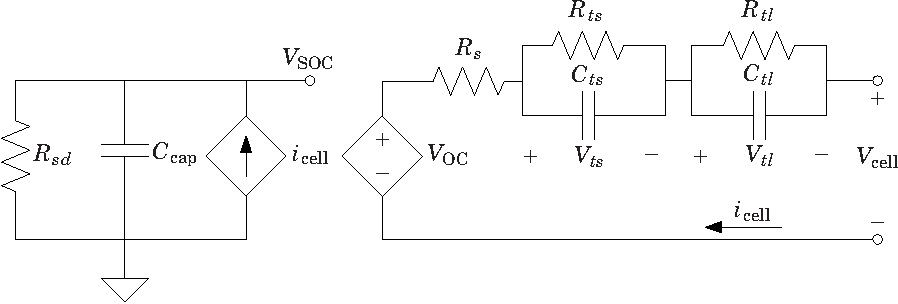
\includegraphics[width=0.9\textwidth]{batt_model}
\caption{Battery model for simulation. [From paper, will redo later]}
\label{fig:batt_model}
\end{figure}

This study used the nonlinear parameters given by Chen and Rinc\'on-Mora for the implementation of a battery using their battery model in Matlab. \emph{The other, constant parameters were chosen to produce a capacity of 4~Ah and a self-discharge rate of 4\% per month, assuming a nominal voltage of 3.7~V. [I didn't properly derive the following equations so my actual values are different.]} To do so, the equivalent capacitance $C_\text{cap}$ to deliver the desired capacity is calculated, and then the resistance $R_{sd}$
that produces the desired self-discharge rate is calculated. 

\textbf{Some errors to be removed:}
{\color{red}
More specifically, the capacitance $C_\text{cap}$ is chosen to so that it supplies the same energy as a battery when discharged at
\begin{equation}
    I_t\,[\text{A}] = C_n\,[\text{Ah}] / 1\,[\text{h}],
\end{equation}
where $I_t$ is the discharge current in amperes, $C_n$ is the rated capacity in ampere-hours, and $n$ is the time base in hours for which the rated capacity is declared~\cite{iec61434,linden01_ch3}. Note that by definition, a fully charged battery with capacity $C_n$ is fully discharged in $n$ hours when discharged at a constant current of $I_t/n$~\cite{linden01_ch3}. The energy delivered by the battery over the $T=n$~hours is then
\begin{align}
    E_\text{batt} &= \int_0^T V(t) I(t) \,\mathrm{d}t = T \left( \frac{1}{T} \int_0^T V(t)\,\mathrm{d}t \right) \frac{I_t}{n} = V_n I_t (1\,\text{h}) \\
    &= 3600 V_n I_t (\text{s}) \,[\text{J}],
\end{align}
where $V_n$ is the nominal voltage. The energy stored in the capacitor $C_\text{cap}$ is $E_\text{cap} = C_\text{cap} V_\text{SOC,max}^2 / 2$. Recall that $V_\text{SOC}$ has a maximum voltage of 1~V, so the capacitance needs to be
\begin{equation}
    C_\text{cap} = 2E_\text{batt}/(1\,\text{V}^2) = 7200 V_n I_t (\text{s}/\text{V}^2) \,[\text{F}]
\end{equation}
}

More specifically, the capacitance $C_\text{cap}$ is chosen so that the charge it holds when $V_\text{SOC}$ equals its maximum of 1~V is equivalent to the capacity of the battery. Therefore, for a given capacity of $C^\dag$ in Ah, $C_\text{cap}$ needs to be
\begin{equation}
    C_\text{cap} = \frac{Q}{V_\text{SOC}} = \frac{C^\dag}{1~\text{V}} = 3600 C^\dag \,[\text{F}].
\end{equation}
Then, the resistance $R_{sd}$ is chosen so that the time constant $\tau=RC$ results in the desired drop of $\xi=0.04$ over $T=1$~month as follows
\begin{gather}
    V(t) = V_0 e^{-T/\tau} = V_0 (1-\xi) \\
    \tau = -T/\ln(1-\xi) = -2592000/\ln 0.96 \,[\text{s}].
\end{gather}
Then, $R_{sd}=\tau/C_\text{cap}$. Thus, the parameters are $C_\text{cap}=14.4$~kF and $R_{sd}=4409.4~\Omega$. \emph{[Actual values used in study are $C=3789.5$ and $R=6290.7$. That works out to 1052.6~mAh and 10.3\% per month. Question is whether to change original setup or redo simulations.]}

For ease of filter design, it is useful to derive the state-space representation of the battery model. The physical variable definition is used, where the state variables are chosen to represent the stored charge in each capacitor. Choosing $x_1=C_{ts}V_{ts}$, $x_2=C_{tl}V_{tl}$, and $x_3=C_\text{cap}V_\text{SOC}$, where the voltages are as defined in \autoref{fig:batt_model}, achieves the goal. Additionally, it can be seen that the cell current influences the state variables, while the
cell voltage is influenced by them. Therefore, $i_\text{cell}$ is defined as the state input and $V_\text{cell}$ is defined as the state output. The resulting state space representation is
\begin{gather}
    \dot{\mathbf{x}} = \begin{bmatrix}
        -1/R_{ts}C_{ts} & 0 & 0 \\
        0 & -1/R_{tl}C_{tl} & 0 \\
        0 & 0 & -1/R_{sd}C_\text{cap}
    \end{bmatrix} \mathbf{x} + \begin{bmatrix} 1 \\ 1 \\ -1 \end{bmatrix} i_\text{cell} \\
    V_\text{cell} = V_\text{OC} - \frac{x_1}{C_{ts}} - \frac{x_2}{C_{tl}} - R_s i_\text{cell}.
\end{gather}
While the above appears to be a linear system, remember that many of the parameters are functions of $V_\text{SOC}$, and thus, depend on the state $x_3$. Therefore, this is a nonlinear system.

In order to simulate the continuous-time system shown above, it is useful to convert the system to discrete time. For a system with a sample period of $T$ and a system in the form of
\begin{equation}
    \begin{cases}
        \dot{x} = Ax + Bu \\
        y = Cx + Du
    \end{cases},
\end{equation}
the discretization is $A_d=e^{AT}$ and $B_d=A^{-1} (A_d-I) B$ for nonsingular $A$, where $I$ is the identity matrix. Note that $A_d$ and $B_d$ are functions of the SOC. For this nonlinear system, the most reliable numerical method of calculating the necessary exponential of a matrix was found through trial to be using the eigenvalues and eigenvectors. To do so, given a matrix $A$, the matrix exponent is
\begin{equation}
    \text{\emph{to add later}}
\end{equation}
The reliability of this method comes from the full set of eigenvectors resulting from the differing time constants in the system.

%To better determine the necessity of nonlinear filtering for thus system, it is useful to determine the degree of nonlinearity. Recent work in quantizing the degree of nonlinearity was conducted by

\section{Filter Implementations}

%As was seen in the last section, the degree of nonlinearity of the battery model necessitates the use of a nonlinear filter. However, for SOC$>0.2$, the dynamics behave approximately linearly, because the resistance and capacitance parameters are approximately constant. Since the battery operates in this ``linear'' region for the majority of the time, it is useful to compare the performance of a linear filter to the nonlinear filters discussed in \autoref{sec:nl_filt}.

%In order to determine the necessity of incorporating the nonlinear relationship between $V_\text{SOC}$ and $V_\text{OC}$ in the filter design, the linearized right-hand circuit with $V_\text{SOC}=0.6$~V and the left-hand circuit were processed by a Kalman filter in each iteration and in that order, with the nonlinearity calculated implicitly.
% the left-hand circuit along with the right-hand circuit linearized at $V_\text{SOC}=0.6$~V were consecutively processed by the Kalman filter in each itera

\section{Simulation Setup}

Determing the battery states is most difficult under high charge/discharge rates, for which the rate-capacity effect is the strongest. Additionally, idle periods following high currents produce strong recovery effects. Therefore, in order to create the most nonlinear behavior to test the filter performance, pulses were used to charge and discharge the simulated battery. Initially, the battery starts fully discharged and stays idle for 900~s. Then, it is charged to full by charging at 0.25~A for
1900~s. Next, six cycles of discharging and charging are conducted. Each cycle lasted for 28000~s. The pulses had an on-time of 1450~s and an off-time of 1350~s at a current of 0.25~A. It is assumed that the simulated battery has circuitry that keeps the SOC within its limits of zero and one by changing the current flow. This was implemented by a current control scheme that changed the current to the self-discharge rate whenever charging of a full battery or discharging of an empty battery occured.

Because of the possibility of the activation of the current control scheme, it is necessary to first determine the actual current as related to the capacity change within the battery. To do so, the SOC was simulated using the left part of the battery model at various sample rates for the described current, with the described current control scheme, using the \texttt{ode45} solver in Matlab~2013a. To ensure convergence, the max time step was set to the one-tenth of the pulse period.
Additionally, the relative and absolute tolerances were reduced to $10^{-6}$ and $10^{-10}$, respectively, for the same reason. The SOC was found at the sample times using linear interpolation. Afterwards, the numerical central difference of the SOC voltage is found to determine when the current control scheme was active. Then, the current was adjust using this information to represent the actual capacity change within the battery. This adjusted current was used to calculate the actual
SOC analytically, since the left circuit is a LTI system. Following this, the parameters of the right part of the circuit can be calculated as a function of SOC. That part of the system was simulated assuming cubic interpolation of the parameter values using the \text{ode15s} solver with relative and absolute tolerances of $10^{-6}$ and $10^{-10}$. The solver and tolerances were chosen to achieve good accuracy for the stiff system. Finally, the battery voltage is calculated using the
states of the right-hand circuit.

The simulated current and voltage have white Gaussion noise added to them to simulate additive measurement noise.

\begin{figure}
\centering
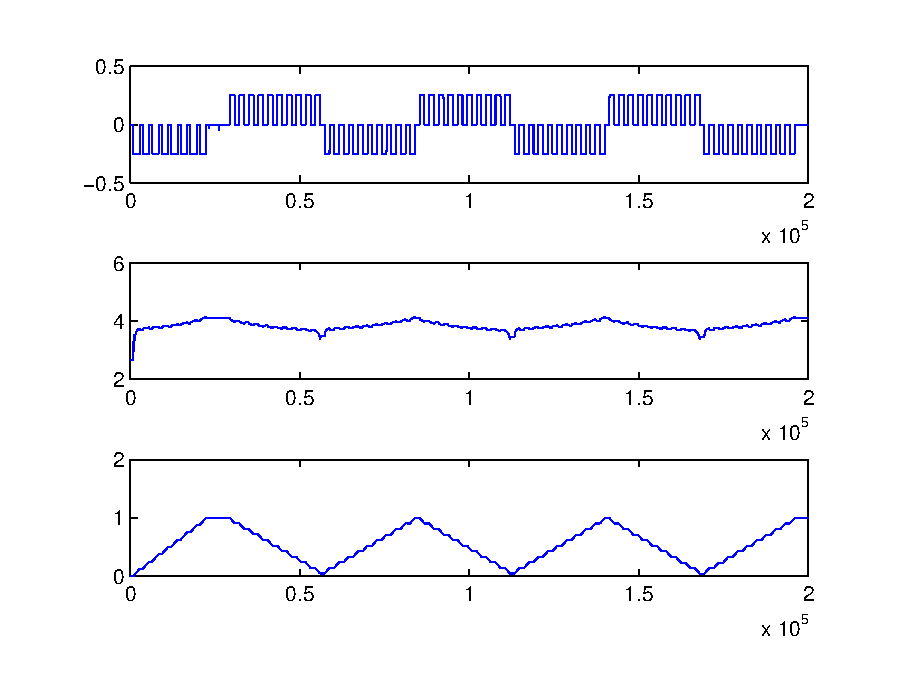
\includegraphics[width=0.9\textwidth]{sim_ideal}
\caption{Discharge current along with the resulting voltage and SOC.}
\label{fig:idealsim}
\end{figure}

\end{document}

\documentclass[../zhang_thesis.tex]{subfiles}
\begin{document}

\chapter{Results}

%%%%%%%%%%%%%%%%%%%%%%%%%%%%%%%%%%%%%%%%%%%%%%%%%%%%%%%%%%%%%%%

For a sampling period of $T_s=90,300$~s, refinement steps of $M=1,2,\dots,2^5$ were used. The filtering was performed assuming an initial state of $x_0=[1,0,0]^\top$ and an initial covariance matrix of $P_0=10^{-6} I_3$, where the initial state was chosen to match the actual state and the initial covariance was experimentally tuned for fast convergence. For the 100 Monte Carlo trials and the four filters, the number of divergences were counted, where a divergence is considered an absolute error in the estimated SOC greater than $0.1$~V or any failure in the filtering process, such as due to a non-invertible matrix or a non-positive definite covariance matrix. If a failure occurs, no attempt was made to keep filtering the system, and the remainder of
the SOC values are assumed to be zero. Additionally, the mean RMSE (MRMSE) is given, where the squared error for each filter is averaged over
the trials and the square root of the result is averaged time.

\begin{sidewaystable}
\caption{Divergences and MRMSE for various filters at $T_s=90$~s.}
\centering
\begin{tabular}{l*{12}{c}}
\toprule
Filter & \multicolumn{2}{c}{$M=1$} & \multicolumn{2}{c}{2} & \multicolumn{2}{c}{4} & \multicolumn{2}{c}{8} & \multicolumn{2}{c}{16} & \multicolumn{2}{c}{32} \\
\cmidrule(r){2-3} \cmidrule(lr){4-5} \cmidrule(lr){6-7} \cmidrule(lr){8-9} \cmidrule(lr){10-11} \cmidrule(lr){12-13} \\
& Divs. & MRMSE & Divs. & MRMSE & Divs. & MRMSE & Divs. & MRMSE & Divs. & MRMSE & Divs. & MRMSE \\
\midrule
EKF & 100 & 0.4245 &  99 & 0.5044 \\
CKF & 100 & 16202  & 100 & 0.4609 \\
UKF & 100 & 7.4105 & 100 & 980.69 \\
SLF & 100 & 0.3007 & 100 & 0.2253 \\
\bottomrule
\end{tabular}
\end{sidewaystable}

\begin{sidewaystable}
\caption{Divergences and MRMSE for various filters at $T_s=300$~s.}
\centering
\begin{tabular}{l*{12}{c}}
\toprule
Filter & \multicolumn{2}{c}{$M=1$} & \multicolumn{2}{c}{2} & \multicolumn{2}{c}{4} & \multicolumn{2}{c}{8} & \multicolumn{2}{c}{16} & \multicolumn{2}{c}{32} \\
\cmidrule(r){2-3} \cmidrule(lr){4-5} \cmidrule(lr){6-7} \cmidrule(lr){8-9} \cmidrule(lr){10-11} \cmidrule(lr){12-13} \\
& Divs. & MRMSE & Divs. & MRMSE & Divs. & MRMSE & Divs. & MRMSE & Divs. & MRMSE & Divs. & MRMSE \\
\midrule
EKF & 100 & 0.8583 & 100 & 0.4269 & 100 & 0.5213 & 100 & 18.34  &  23 & 0.1247 & 100 & 0.1523 \\
CKF & 100 & 494.4  & 100 & 0.4274 & 100 & 0.3045 & 100 & 0.3044 &  27 & 0.0830 & 100 & 0.1769 \\
UKF & 100 & 248.3  & 100 & 4.061  & 100 & 0.3137 & 100 & 0.3026 &  34 & 0.1141 & 100 & 0.2307 \\
SLF & 100 & 0.2750 & 100 & 0.3038 & 100 & 0.3050 & 100 & 1.3081 & 100 & 0.2099 & 100 & 0.0125 \\
\bottomrule
\end{tabular}
\end{sidewaystable}

\end{document}

%\documentclass[../zhang_thesis.tex]{subfiles}
\begin{document}

\chapter{Discussion}

%%%%%%%%%%%%%%%%%%%%%%%%%%%%%%%%%%%%%%%%%%%%%%%%%%%%%%%%%%%%%%%

In terms of speed, for a given number of integration steps, the EKF is about 3 to 4 times faster than the SLF and 7 times faster than the UKF and CKF. Additionally, the time about doubles for each doubling in the number of integration steps. Note that the majority of the time is spend in performing the numerical integration, so the complexity of the discretization method directly affects the speed. The EKF has the simplest discretization so it is naturally the fastest. The SLF uses the
same method as the EKF but evaluates it multiple times per integration step, so it is somewhat slower. The UKF and CKF use a complex IT-1.5 discretization method that uses the Jacobians and Hessians of the system, so it is the slowest. Evaluation of the discretization at multiple sigma points further slows down these filters. Note that they are very fast for low numbers of integration steps, which can be explained by the filters encountering numerical problems with the Cholesky factorization
and skipping to the next trial.

In terms of the number of divergences, the EKF performs the best for $T_s=30$ seconds with some trials with good accuracy for $M=1$ and 2, followed by the CKF and SLF. The UKF performs the worst, with numerical problems for large $M$. The other three filters have good accuracy for $M\ge 4$. For $T_s=150$ seconds, the SLF has the lowest number of divergences, with good accuracy for $M\ge 8$, while the others need $M\ge 16$. The EKF is the second best with a few good trials at $M=4$ and 8.
The UKF and CKF tie for last place. For $T_s=300$ seconds, the CKF and SLF are the best with good accuracy for $M\ge 16$. The other two need $M\ge 32$, but EKF is slighly better than the UKF with less divergences at $M=16$. Overall, the SLF resulted in the best performance in terms of the number of divergences as a function of the number of integration steps. It achieved zero divergences at a equal or smaller number of integration steps for each of the sampling periods. The EKF and
CKF are close behind in performance. The EKF was able to get fewer than 100 divergences for $T_s=30$ and 150, where the CKF had 100 divergences. However, at $T_s=300$, the CKF achieves zero divergences at a smaller $M$ value. The worst performing filter was the UKF which had the highest number of divergences. In addition, it had some divergences for $T_s=30$ seconds for $M=128$ and 256, probably caused by numerical problems related to the unscented transform.

In terms of the MRMSE, for $T_s=30$ seconds, the EKF, CKf, and SLF are about equal in performance for $M\ge 4$, at which the divergences are zero. The MRMSE is flat in that range for those three filters. The best accuracy is achieved by the CKF at $M=32$. The UKF has poor performance at this sample rate and diverges for $M\ge 128$. For $T_s=150$ seconds, the SLF achieves the best performance for $M\le 8$, and the EKF has the worst performance. The CKF and UKF are about equal over the
range, with the UKF being significantly better at $M=1$. Larger values of $M$ shown increases in accuracy for all the filters, with the EKF achieving the best accuracy for $M\ge 16$. The CKF and SLF are about equal over the same range, while the UKF has the worst accuracy. For $T_s=300$ seconds, the SLF achieves the best accuracy for $M\le 16$, and the EKF has very poor performance. The CKF and UKF are about equal, with the CKF having a small edge in accuracy. For higher values of $M\ge
32$, the EKF achieves the best accuracy. The CKF and SLF are about equal over the range, and the UKF has the worst accuracy.

It can be seen that the trend of accuracy as a function of the number of integration steps is similar for sample period of 150 and 300 seconds, where the doubling in the number of integration steps at which no divergences are encountered from $T_s=150$ to 300 seconds is explained by the doubling of the sample period. The SLF has the best performance for a small number of integration steps, while the EKF has the best performance for greater than or equal to 16 and 32 integration steps for the sample
periods of 150 and 300, respectively. For a sample period of 30 seconds, the EKF, CKF, and SLF perform equally well for greater than or equal to 4 integration steps, while the UKF encounters numerical problems that cause it to diverge for greater than 64 integration steps.

Overall, the EKF has the best accuracy and the best speed, for sufficiently large numbers of integration steps. The speed is expected since it is the least complex of the studied filters. In addition, its poor performance at small numbers of integration steps is due to the nonlinearity of the system. However, its greater accuracy for large numbers of integration steps is surprising since the battery system is strongly nonlinear, particularly for SOC near zero. This effect could be
caused by a non-Gaussian posterior distribution of the noises, which would negatively impact the Gaussian assumption used by the other filters. The LMMSE Kalman filter does not make such an assumption to minimize the error covariance. In fact, Kalman showed that the linear estimate with non-Gaussian noise can only be improved by nonlinear estimation when at least third-order probability distribution functions are considered~\cite{kalman60}. As this was not the case with the chosen filters, it
makes sense that the EKF performs the best when a sufficiently large number of steps are used to minimize the error of the numerical integration.

\end{document}

%\chapter{Modern Applications}

%%%%%%%%%%%%%%%%%%%%%%%%%%%%%%%%%%%%%%%%%%%%%%%%%%%%%%%%%%%%%%%

Even though faience is an ancient material, it has certain properties not commonly found in modern materials. Its notable properties include self-glazing, low firing temperature, and antimicrobial attributes. The applications of these properties in modern industry are explored in Sections 5.1 through 5.3. The economic and environmental considerations associated with faience technology are described in Section 5.4.

%%%%%%%%%%%%%%%%%%%%%%%%%%%%%%%%%%%%%%%%%%%%%%%%%%%%%%%%%%%%%%%

\section{Applications of Self-Glazing}

Modern ceramics are glazed using a method similar to the application method of glazing associated with faience production. As in faience, this applied glaze can bear drying or firing marks and is prone to runs or drips. These marks can be prevented with the self-glazing methods of faience, of which cementation is better suited as it does not require a granular body unlike efflorescence. In addition, the production process would be simplified as glazing would be done in conjunction with firing.

A method similar to cementation is salt glazing (according to Dr.\ Williamson~\cite{vandiver83}), which was widely used before environmental clean air restrictions led to its demise~\cite{dodd94}. Glazing by cementation may be used in place of salt glazing to produce similar results but without the associated air pollution and with a simpler firing process.

Another use of self-glazing could be to simulate enamels and glazes made using frit, which is similar in composition to faience glaze. There are many modern uses for frit. For example, frits of primarily silica, diboron trioxide, and soda have been used as enamels on steel pipes. However, creating frit is a complicated process that involves fusing the components, quenching them to form glass, and then granulating the glass. The simpler cementation glazing method could be used to produce similar enamels and glazes as with frit.

%%%%%%%%%%%%%%%%%%%%%%%%%%%%%%%%%%%%%%%%%%%%%%%%%%%%%%%%%%%%%%%

\section{Applications of Low Firing Temperature}

Faience has a lower firing temperature ($<$1000$^\circ$~C) than most modern ceramics. Thus, faience could be used in place of modern ceramics when materials sensitive to heat are used.

Current packagings for semiconductor chips are made from ceramics or glass-ceramics. The high heat of the production process necessitates that the semiconductor chips be attached after the ceramic has been made~\cite{tummala91,ivf.se}. Presently, the chips are attached using solder. Solder is harmful to the environment (often lead-based) and less conductive than copper wiring, which restricts operating speeds. Using faience as the package allows the semiconductor chip to be placed prior to firing, eliminating the use of solder.

Additionally, advances have been made in the field of organic semiconductors. Organic semiconductors are of interest due to the low cost of their manufacture---they could theoretically be manufactured using simple inkjet printer techniques~\cite{chiang77}. However, they are very sensitive to heat, which makes them difficult to package using modern ceramics or glass-ceramics. The low heat of faience manufacturing could potentially be used with organic semiconductors.

%%%%%%%%%%%%%%%%%%%%%%%%%%%%%%%%%%%%%%%%%%%%%%%%%%%%%%%%%%%%%%%

\section{Applications of Antimicrobial Properties}

There are many antimicrobial surfaces approved by the EPA. These surfaces use copper or silver alloys, which have certain antimicrobial properties~\cite{epa,coppertouch}. However, no ceramic material has been approved. For aesthetic and practical purposes (e.g.\ tiles), it would be beneficial to have an antimicrobial ceramic material. The obvious choice is faience, which has some antimicrobial properties due to the copper oxide colorant in the glaze. These antimicrobial properties can be improved with cementation or application glazing, which result in thick glazes high in copper oxide.

Faience can be made into tiles for use in such places as hospitals and kitchens. Faience tiles would not only prevent the spread of disease, but also serve a decorative function. Also, the faience glaze may be applied to metals to further improve their antimicrobial properties.

%%%%%%%%%%%%%%%%%%%%%%%%%%%%%%%%%%%%%%%%%%%%%%%%%%%%%%%%%%%%%%%

\section{Economic and Environmental Considerations}

%The coating process of faience is governed by the process of efflorescence, from French meaning ``to flower out''. Efflorescence is a natural occurrence when soluble salts in a ceramic dry to the surface. It is most commonly seen as a white frost on bricks or concrete. As the soluble salt dries, it evaporates out of the ceramic body, leaving a salt powder on the surface. Egyptian faience makes uses of this property of copper salts evaporating as a self-glazing technique.

The use of faience in modern industry would be beneficial both economically and environmentally. Faience production requires fewer steps than traditional ceramics. Reducing steps in processing ceramics leads to an increase in efficiency. This reduction may cause a reduction in energy used creating a lower impact on the environment. Additionally, the low firing temperature of faience also lends to a reduction in energy use.
%Some of the methods used in efflorescence could be applied to modern ceramic technology. Fluxes could be used create gradients to drive alkalis through the ceramic body possibly for composite technology.

Environmentally, faience production uses little energy, which would have been necessary in Egypt, a country devoid of ample fuel. Faience can be used in place of more environmentally damaging processes, such as salt glazing. Additionally, faience is nontoxic---ancient Egyptians would even ingest faience as medicine~\cite{bittle11}.
 
%Fabricating faience coatings may also be a viable alternative to some high tech
%wear or corrosion resistant coatings. It may be similar to the CMAS techniques
%of covering columnar structures with a hard top layer that fills in-between the
%columns. The replicated faience has a copper oxide content of about 3 to 10 weight
%percent. By increasing the copper oxide, to increase efflorescence, improved antimicrobial protection may be achieved.

%If the ceramic has similar anti-microbial protection, while using
%less copper, the cost would come down. Faience is comprised of mostly quartz
%which is easily acquired at low cost. The benefit of Tite's method of recreating faience, is that it can be done by hand, but the properties and thickness of the coating leave room for improvements. The copper oxides do not effloresce to the surface as much as the authentic Egyptian faience. Lost to time are ancient processing techniques that may be useful for current industry.

%Certain metals and alloys, like copper, silver and bronze have been approved as
%alloys for antimicrobial purposes in public health products (EPA 1). No ceramic
%based material has been approved. Copper salts may bind to fungal enzymes and
%causes K+ ions to release [26]. This technique may not be better than pure copper alloys for their antimicrobial properties, but the ceramic may have other sought-after characteristics. For instance, the ceramic could be made into tile flooring, whereas metallic flooring is relatively unheard of since it is slippery, expensive and not aesthetically appealing. The goal of creating an anti-microbial ceramic tile is within reach.

%The reason for creating faience is unclear. The materials used to create faience were readily available and may have happened by mistake. Faience is relatively easy to recycle and recreate new lower quality faience. It may also be possible to harvest the copper through leaching in aqueous processing. Since Egyptian faience doesn't require high quality materials, recycled copper and copper alloys maybe applicable for use.

%In the New Kingdom, faience may have been used to simulate lapis lazuli. Faience was lightweight enough to wear around the extremities whereas turquoise, lapis lazuli, malachite and azurite may have been harder to carve and heavier on the skin.
%\chapter{Conclusions and Future Work}

%%%%%%%%%%%%%%%%%%%%%%%%%%%%%%%%%%%%%%%%%%%%%%%%%%%%%%%%%%%%%%%

\section{Summary}

This thesis confirmed the results of previous investigations. In particular, the 22nd Dynasty Abydos faience beads of this study have compositions and microstructures similar to the beads in the 2007 study by Tite \emph{et al.}\ with the same distinctions (time period and production site). Similar conclusions on the raw materials and glazing method were reached by both investigations.

This thesis also improved upon previous studies by employing new techniques. Compositional mappings were made that showed the concentration of each element over an area of the faience. This technique allows the investigator to easily notice how the concentration of certain elements change in two dimensions and not just one. In addition, an attempt was made to analyze the unglazed inner surface found in faience beads. While some differences between it and the body were noted, the cause of these differences was not determined.

Lastly, this thesis explored potential modern applications for faience technology. It was determined that there are areas that could benefit from the technology of faience. The economic and environmental considerations of faience usage were also determined.

%%%%%%%%%%%%%%%%%%%%%%%%%%%%%%%%%%%%%%%%%%%%%%%%%%%%%%%%%%%%%%%

\section{Future Work}

Future studies of faience will need to consider three factors: the time period, the production site, and the specific type of object. This study and previous ones~\cite{vandiver83,vandiver98,tite07} have noted how these factors can greatly impact the composition and microstructures of faience. However, it would be difficult for one study to have diversity in each of these areas. Therefore, another recommendation is that future researchers need to collaborate in order to map the entire spectrum of faience.

A different area of study is the replication of faience, which still needs a lot of research. Future replication studies should focus on hybrid glazing methods to better understand how ancient faience was glazed. Furthermore, replication studies need to consider the wide range of colors found in ancient faience.

Additionally, modern applications of faience technology should be further explored. Conversely, current nanotechnology could be used to improve faience by increasing the quality of the raw materials to allow for better glazing.

%This thesis set the framework for future work by demonstrating that there is more to learn about faience. Future work should be more of a quantitative nature and should apply the techniques of this study to a wider range of faience objects. In particular, the impurities in faience can be used to locate the exact source of the raw materials of faience.

%Future work should also investigate reproducing faience. Little is known about the mechanisms behind glaze formation, particularly in the cementation method. In-depth knowledge of the glazing process gained from reproducing faience could potentially be used to improve modern ceramic technology. Additionally, faience could have direct uses as a water-resistant, antimicrobial material.

%Future work may include varying the particle size and distribution of the powders in recreating Egyptian faience to understand the exact processing conditions. Recent studies by Mimi Leveque suggest that adding gum-Arabic will aid in removing the faience from molds (Nicholson in Friedman's book 51).
%
%The next step in analyzing Ancient faience may be to separate the glaze from the body and perform XRD to determine the individual crystal structures.
%
%Compile a map of provenance for the different sand compositions of the Egyptian faience, building on Kaczmarcsyk and Hedges exploration of different regional techniques (Kaczmarcsyk and Hedges 5).
%
%Differences that arise from size of the faience, the difference between beads and shabti figurines, has also largely gone unstudied (Kaczmarcsyk and Hedges 9).
%%%%%%%%%%%%%%%%%%%%%%%%%%%%%%%%%%%%%%%%%%%%%%%%%%%%%%%%%%%%%%%
% Appendices
%
% Because of a quirk in LaTeX (see p. 48 of The LaTeX
% Companion, 2e), you cannot use \include along with
% \addtocontents if you want things to appear the proper
% sequence. Since the PSU Grad School requires 
%%%%%%%%%%%%%%%%%%%%%%%%%%%%%%%%%%%%%%%%%%%%%%%%%%%%%%%%%%%%%%%
%\appendix
%%\Appendix{Vita}

\begin{singlespace}
%\setlength{\parskip}{\baselineskip}
%\newlength{\vitaskip}
%\setlength{\vitaskip}{-22pt}
%\newlength{\vitaitemsep}
%\setlength{\vitaitemsep}{-3.5pt}

The author was born in Nanjing, China. He obtained his Bachelor's of Science in electrical engineering from the Pennsylvania State University in 2011. He attended the University of New Orleans to pursue a Master's of Science in electrical engineering, and performed research with Dr. Huimin Chen.
\end{singlespace}
%%%%%%%%%%%%%%%%%%%%%%%%%%%%%%%%%%%%%%%%%%%
} % End of the \allowdisplaybreak command %
%%%%%%%%%%%%%%%%%%%%%%%%%%%%%%%%%%%%%%%%%%%

%%%%%%%%%%%%%%%%
% BIBLIOGRAPHY %
%%%%%%%%%%%%%%%%
% You can use BibTeX or other bibliography facility for your
% bibliography. LaTeX's standard stuff is shown below. If you
% bibtex, then this section should look something like:
\clearpage
   \begin{singlespace}
	 \phantomsection
   \bibliographystyle{FG-bibstyle}
   \addcontentsline{toc}{chapter}{Bibliography}
   \bibliography{Biblio-Database}
   %\printbibliography
   \end{singlespace}

%\allowdisplaybreaks{
%\appendix
%%\Appendix{Vita}

\begin{singlespace}
%\setlength{\parskip}{\baselineskip}
%\newlength{\vitaskip}
%\setlength{\vitaskip}{-22pt}
%\newlength{\vitaitemsep}
%\setlength{\vitaitemsep}{-3.5pt}

The author was born in Nanjing, China. He obtained his Bachelor's of Science in electrical engineering from the Pennsylvania State University in 2011. He attended the University of New Orleans to pursue a Master's of Science in electrical engineering, and performed research with Dr. Huimin Chen.
\end{singlespace}
%}

\nocite{*}

\backmatter

% Vita
%\phantomsection
%\addcontentsline{toc}{chapter}{Vita}
%\vita{SupplementaryMaterial/Vita}

\end{document}

